\chapter{Results and Discussion}\label{sec:resultsanddiscussion}

Some more general text
Why are some parts simulating and some parts using IBM?

\section{Simulating the qubit-based kNN algorithm}
\label{subsec:qubitKNNresults}

Introduce a 9-bit RGB colour classification problem!

The computer used for the Liqui$\ket{}$ quantum simulations in this thesis only provides 8GB of RAM limiting the maximum number of simulated qubits to 24. Unfortunately, real-world machine learning problems usually involve large datasets that would require much more qubits a small artificial dataset needs to be constructed. For this reason, the classification of 9-bit, little-endian RGB colour codes will be considered.

The training data set is shown in Table ? and consists of three red and three blue 9-bit RGB colour codes.

\begin{table}
    \begin{tabular}{| c| c |c |}
      %\toprule
      Colour & Binary 9-bit RGB string & Class\\
      \midrule
       \cellcolor{red1} & 111 000 000 & Red ($\ket{0}$)\\\midrule
       \cellcolor{red2} & 101 000 000 & Red ($\ket{0}$)\\\midrule
       \cellcolor{red3} & 110 000 000 & Red ($\ket{0}$)\\\midrule
       \cellcolor{blue1} & 000 000 111 & Blue ($\ket{1}$)\\\midrule
       \cellcolor{blue2} & 000 000 101 & Blue ($\ket{1}$)\\\midrule
       \cellcolor{blue3} & 000 000 100 & Blue ($\ket{1}$)\\\midrule
      \bottomrule
    \end{tabular}
    \caption{Training data set of six 9-bit RGB colour codes}
\end{table}

\begin{table}
    \begin{tabular}{| c| c |c |}
      %\toprule
      Colour & Binary 9-bit RGB string & Class\\
      \midrule
       \cellcolor{redinput} & 111 000 000 & Red ($\ket{0}$)\\\midrule
       \cellcolor{blueinput} & 101 000 000 & Red ($\ket{0}$)\\\midrule
      \bottomrule
    \end{tabular}
    \caption{Input data set of two 9-bit RGB colour codes}
\end{table}

Implementation of Trugenberger Storage

The first step towards simulating the qubit-based kNN algorithm proposed by \citeA{Schuld2014} as described in detail in Section~\ref{subsubsec:quantumknearestneighbour} is preparing the initial superposition over all training vectors:

\begin{equation}
\ket{T} = \frac{1}{\sqrt{N}}\sum_{p=1}^N \ket{v_1^p,v_2^p,...v_n^p;c^p}
\end{equation}

This can be done using the quantum state preparation algorithm by \citeA{Trugenberger2001} outlined in Section~\ref{subsubsec:classicaldataqubits}. First, the training feature vectors $v_1,v_2,...,v_n$ containing classical data are first reexpressed 

redefine the $m$ register from Equ.~\ref{} as the 

Combined implementation of Trugenberger Storage and Schuld qubit kNN

More concrete example needed!

\newpage

\section{Development of an amplitude-based kNN algorithm}
\label{subsec:amplitudeKNNresults}

IBM doesn't allow for qubit based kNN due to restriction in qubit number

need for a new algorithm based on amplitudes

\begin{equation}
\frac{1}{\sqrt{2M}}\sum_{m=1}^{M} (\textcolor{emerald}{\ket{0}}\ket{\textcolor{red}{\Psi_{\tilde{x}} (\star)}}+\textcolor{emerald}{\ket{1}}\ket{\textcolor{darkyellow}{\Psi}_{\textcolor{purple}{x^{m}}}})\ket{y^{m}(\textcolor{darkyellow}{A} \ or \ \textcolor{purple}{B})}\ket{m}
\end{equation}
where
\begin{equation}
\ket{\textcolor{red}{\Psi_{\tilde{x}} (\star)}} = \sum_{i=1}^{N} \textcolor{red}{\tilde{x}_i}\ket{i} \quad \quad
\ket{\textcolor{darkyellow}{\Psi}_{\textcolor{purple}{x^{m}}}}	 = \sum_{i=1}^{N} \textcolor{darkyellow}{x}\textcolor{purple}{_i^m} \ket{i} 
\end{equation}

\begin{equation}
e.g. \quad \begin{pmatrix}
 \textcolor{blue}{0.6} \\ 
 \textcolor{emerald}{0.4}
 \end{pmatrix} \quad \rightarrow \quad \ket{n} =  \sqrt{\textcolor{blue}{0.6}}\ket{0}+\sqrt{\textcolor{emerald}{0.4}}\ket{1}
\end{equation}

Applying the \textbf{Hadamard gate} interferes the input and the training vectors:

\begin{equation}
\frac{1}{2\sqrt{M}}\sum_{m=1}^{M} (\textcolor{emerald}{\ket{0}}[\ket{\textcolor{red}{\Psi_{\tilde{x}}}}+\ket{\textcolor{darkyellow}{\Psi}_{\textcolor{purple}{x^{m}}}}]+\textcolor{emerald}{\ket{1}}[\ket{\textcolor{red}{\Psi_{\tilde{x}}}}-\ket{\textcolor{darkyellow}{\Psi}_{\textcolor{purple}{x^{m}}}}])\ket{y^{m}(\textcolor{darkyellow}{A} \ or \ \textcolor{purple}{B})}\ket{m}
\end{equation}

$\rightarrow$ Perform \textbf{conditional measurement} on ancilla qubit.\\
Successful if $\ket{0}$ state is measured.

After successful conditional measurement, the state is proportional to
\begin{equation}
\frac{1}{2\sqrt{M}}\sum_{m=1}^{M} \sum_{i=1}^{N} (\textcolor{red}{\tilde{x}_i}+\textcolor{darkyellow}{x}\textcolor{purple}{_i^m})\ket{0}\ket{i}\ket{y^{m}(\textcolor{darkyellow}{A} \ or \ \textcolor{purple}{B})}\ket{m}
\end{equation}

Probability to measure class B:
\begin{equation}
p(\ket{y^m} = \ket{1(\textcolor{purple}{B})})= \sum_{m \mid y^m=1(\textcolor{purple}{B})} 1 - \frac{1}{4M} \mid \textcolor{red}{\tilde{x}} - \textcolor{purple}{x^m} \mid ^2
\end{equation}

Hereby, the advantages of the quantum version are the parallel computation of the distances between each training vector and the input vector as well as contracting distance computation and distance weighting into one computational step.

The quantum advantage of the algorithm is the simultaneous computation of the HD between the input vector and each training vector which is impossible to do classically. For example, if the training set contains 1,000,000 vectors with 10 entries each, the quantum algorithm performs all 1,000,000 distance computations with the application of only 10 X and 10 CNOT gates. In contrast, the classical algorithm would need to perform  1,000,000 individual computations in order to be able to apply distance-dependent weights to each training vector. 

\subsubsection{Diffusion matrix from quantum random walks}
\label{subsubsubsec:diffusion}

Initialization of amplitude distribution is non-trivial

Need for a simpler way - using diffusion matrix from quantum random walks

For the simplest case, consider the entries in the classical probability vector v to be normal distributed, e.g.

CHECK THE ORDER!
\begin{equation}
v = \colvec{0.064180\\0.146860\\0.146770\\0.341590\\0.026840\\0.063590\\0.061700\\0.148470}
\end{equation}

The goal is to encode this classical data into a quantum memory state $\ket{M}$ of the form,

\begin{align}
\ket{M} = \quad &0.064180 \ket{000} +
0.146860 \ket{100} +
0.146770 \ket{010} +
0.341590 \ket{001}\notag\\
&+ 0.026840 \ket{110}
+ 0.063590 \ket{011} +
0.061700 \ket{101} +
0.148470 \ket{111}
\end{align}

%Before outlining how to prepare state $\ket{M}$ the notion of Hamming distance needs to be introduced.

Furthermore, a useful tool of visualizing the HDs between binary patterns made from three qubits is a 3-D cube as shown in Fig.~\ref{img:cubenoprobs}. On the cube, adjacent qubit patterns have a HD of 1 and the HD increases by 1 for every additional corner. For example, the qubit state $\ket{000}$ is adjacent to $\ket{100}$ since they only differ in one qubit ($HD=1$). Moving one more corner yields the state $\ket{101}$ or $\ket{110}$ which both have a HD of 2 compared to $\ket{000}$.

\begin{figure}[!ht]
       \centering
       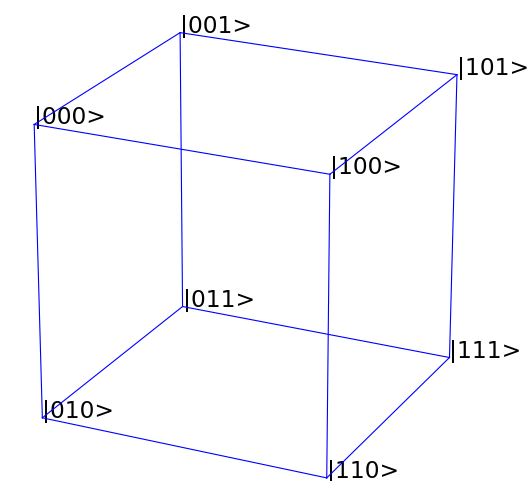
\includegraphics[width=0.5\textwidth]{img/cubewithoutprobs.png}
       \caption{\label{img:cubenoprobs} Visualizing Hamming distances on a 3-D cube}
\end{figure}

This way of visualizing HDs can be extended to the 16 binary patterns made by four qubits that can be visualized on a 4-D cube, also called tesseract, as illustrated in Fig.~\ref{img:hypercubenoprobs}.

\begin{figure}[!ht]
       \centering
       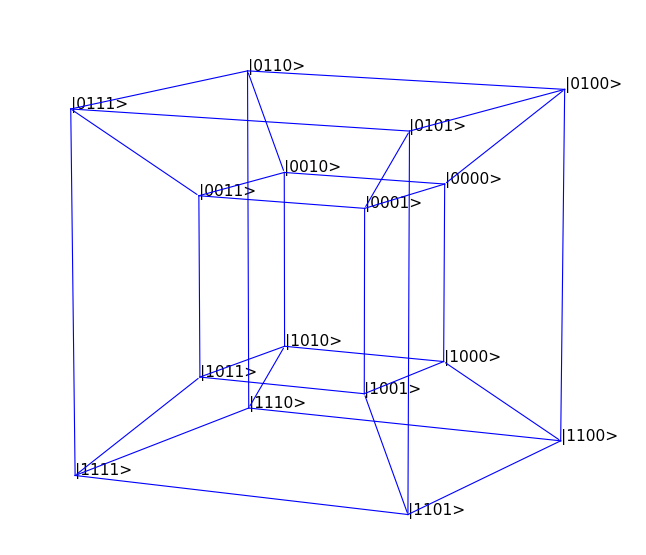
\includegraphics[width=0.5\textwidth]{img/hypercubewithoutprobs.png}
       \caption{\label{img:hypercubenoprobs} Visualizing Hamming distances on a 4-D cube (tesseract)}
\end{figure}

The idea of a coin operator $C$ can be borrowed from the theory of quantum random walks to initialize a gaussian distribution centered around a chosen binary qubit pattern. For this purpose, the coin operator is defined as,

\begin{equation}
C = \begin{pmatrix}
\sqrt{\delta} & 1-\sqrt{\delta} \\
1-\sqrt{\delta} & -\sqrt{\delta}
\end{pmatrix}
\end{equation}

where $0 \leq \delta \leq 1$.

IBM implementation problems

Complexity analysis of actual implementation with IBM QC

\subsubsection{Controlled U Gate}
\label{subsubsubsec:controlledugate}

Often there is a need for applying certain quantum gates in a controlled manner. Thus a controlled U (CU) gate is required whereby U can be any unitary single-qubit gate. The CU gate is defined as:

\begin{equation}
CU = \begin{pmatrix}
 \mathbb{1} & 0 \\ 
 0 & U
 \end{pmatrix}
\end{equation}

It is important to note that the CNOT gate is essentially a CU gate in the case of U = X. 

Most of the time the CU gate cannot be implemented directly and has to be realized through larger quantum circuits consisting of CNOT and single-qubit gates. \citeA{nielsen2010quantum} describe such a decomposition as shown in Fig.~\ref{img:cudecomposition}.

\begin{figure}[ht]
   \centering
   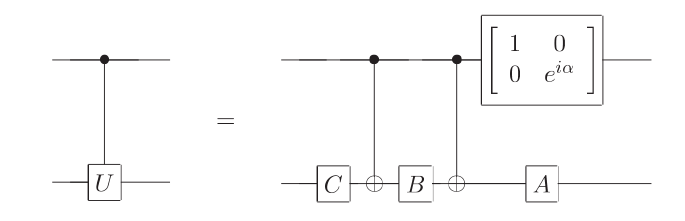
\includegraphics[width=0.7\textwidth]{img/controlledudecomp.png}
   \caption{Circuit decomposition for a controlled-U operation for single-qubit gate U.\textsuperscript{3}}
   \label{img:cudecomposition}
\end{figure}

\footnotetext[3]{Reprinted from Michael A. Nielsen and Isaac L. Chuang. Quantum Computation and Quantum Information. Cambridge University Press, 2000. Copyright 2010 by Nielsen \& Chuang.}

The idea is that when the control qubit is \0 the gate combination ABC is applied to the target qubit and has to equal the identity gate:

\begin{equation}
ABC = \mathbb{1}
\end{equation}

If and only if the control qubit is \1 then the gate sequence $e^{i\alpha}AXBXC$ is applied to the target. Since the goal is to apply the unitary U to the target qubit the following equation must be satified,

\begin{equation}
e^{i\alpha}AXBXC = U
\end{equation}

In order to find the matrices A,B,C and the additional parameter $\alpha$ the following equation has to be solved:

\begin{equation}
U = \begin{pmatrix}
 e^{i(\alpha-\frac{\beta}{2}-\frac{\delta}{2})}\cos{\frac{\gamma}{2}} & -e^{i(\alpha-\frac{\beta}{2}+\frac{\delta}{2})}\sin{\frac{\gamma}{2}} \\ 
e^{i(\alpha+\frac{\beta}{2}-\frac{\delta}{2})}\sin{\frac{\gamma}{2}} & e^{i(\alpha+\frac{\beta}{2}+\frac{\delta}{2})}\cos{\frac{\gamma}{2}}
 \end{pmatrix}
\end{equation}